\begin{enumerate}
 \item On calcule les racines carrées de $4-3i$ par la méthode du cours puis on multiplie par $\sqrt{2}$. On en tire que les racines carrées de $8-6i$ sont $3-i$ et $-3+i$.\newline
Les antécédents de $1+i$ par $f$ sont $2$ et $-1+i$.\newline
En effet, ce sont les solutions de l'équation d'inconnue $z$
\begin{displaymath}
 \frac{z^2}{z-2i}= 1+i \Leftrightarrow z^2 -(1+i)z +2(-1+i)=0
\end{displaymath}
Le discriminant de cette équation du second degré est $8-6i$ dont on a calculé les racines. On en déduit les antécédents.

\item On se propose de montrer que :
\begin{itemize}
 \item si $h\in\{0,8i\}$, $h$ admet un seul antécédent.
 \item si $h\not\in\{0,8i\}$, $h$ admet deux antécédents distincts.
\end{itemize}
En effet la recherche d'un antécédent de $h$ par $f$ se traduit par $f(z)=h$ c'est à dire l'équation du second degré
\begin{displaymath}
 z^2 -hz +2ih = 0
\end{displaymath}
dont le discriminant est $\Delta = h^2-8ih = h(h-8i)$.\newline
 L'étude de la surjectivité et de l'injectivité de la fonction revient à celle de l'équation d'inconnue complexe $z$
\begin{displaymath}
  f(z) = h \Leftrightarrow z^2 = (z-2i)h
\end{displaymath}
que l'on vient d'étudier. Elle admet \emph{toujours} des solutions pour n'importe quel paramètre $w$. La fonction est donc \emph{surjective}.\newline
En général (sauf si le discriminant est nul), cette équation admet deux solutions \emph{distinctes}: la fonction \emph{n'est donc pas injective}.

\item Le calcul des parties réelles et imaginaires de $g(z)$ conduit à :
\begin{align*}
 \Re g(z) =2x^3 -2xy^2-4xy & & \Im g(z) = 4x^2y +2x^2 -2y^2
\end{align*}

En effet
\begin{displaymath}
 g(z)= z^2(\overline{z}+2i)+z^3 = |z|^2z+2iz^2 +z^3
\end{displaymath}
Le calcul se termine en exprimant à part les parties réelles et imaginaires de $z^2$ et $z^3$.

\item 
\begin{enumerate}
  \item D'après la question précédente, $g(z)$ est imaginaire pur si et seulement si
\begin{displaymath}
 2x(x^2-y^2-2y)=0
\end{displaymath}
L'ensemble des points dont l'affixe $z$ est tel que $g(z)$ soit imaginaire pur est donc la réunion de la droite $\Delta$ d'équation $x=0$ privée du point $2i$ en lequel la fonction n'est pas définie et de l'ensemble $\mathcal{C}$ d'équation 
\begin{displaymath}
 x^2-y^2-2y=0 
\end{displaymath}

  \item Les affixes $a$, $u_1$ et $u_2$ du point $A$ des vecteurs $\overrightarrow{u_1}$ et $\overrightarrow{u_2}$ sont
\begin{displaymath}
  a = -i,\hspace{0.5cm} u_1 = \frac{1}{\sqrt{2}}(1+i),\hspace{0.5cm} u_2 = \frac{1}{\sqrt{2}}(-1+i)
\end{displaymath}
Comme $|u_1| = |u_2|=1$ et $iu_1=u_2$, le repère $\mathcal{R}'$ est orthonormé direct.\newline
Le calcul des coordonnées se fait avec les affixes. On cherche les réels $X$ et $Y$ tels que 
\begin{displaymath}
  x + iy = a + Xu_1 + Yu_2 \Leftrightarrow
\left\lbrace 
\begin{aligned}
  &x = \frac{1}{\sqrt{2}}\left( X - Y\right) \\ 
  &y = -1 + \frac{1}{\sqrt{2}}\left( X + Y\right)
\end{aligned}
\right. 
\Leftrightarrow
\left\lbrace 
\begin{aligned}
  &X = \frac{1}{\sqrt{2}}\left( x + y + 1\right)\\
  &Y = \frac{1}{\sqrt{2}}\left( -x + y + 1\right)
\end{aligned}
\right. 
\end{displaymath}
  \item On transforme l'équation de $\mathcal{C}$ comme nous y invite l'énoncé:
\begin{multline*}
  x^2 - y^2-2y = 0 \Leftrightarrow x^2 - (y+1)^2 +1 = 0 \Leftrightarrow
  (y+1)^2-x^2 = 1  \\ \Leftrightarrow (y+1+x)(y+1-x) = 1
  \Leftrightarrow 2XY = 1
\end{multline*}
L'ensemble $\mathcal{C}$ est donc formé par les points de coordonnées $(t,\frac{1}{2t})$ dans le repère $\mathcal{C}$. Il s'agit d'une hyperbole.
\end{enumerate}
\begin{figure}[h]
  \centering
  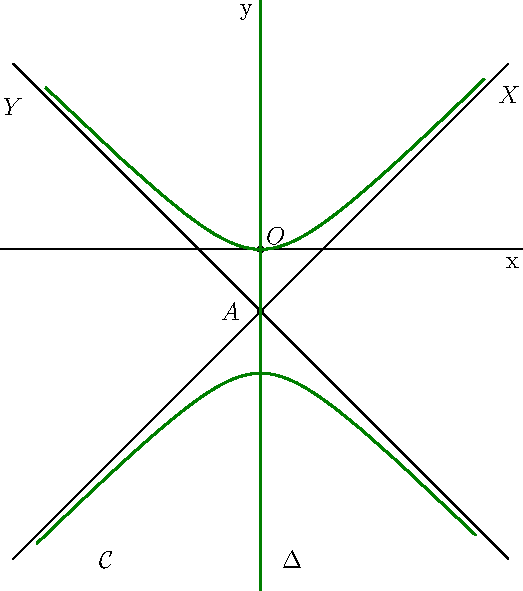
\includegraphics{./Ccomp5_1.pdf}
  % Ccomp5_1.pdf: 0x0 pixel, 0dpi, 0.00x0.00 cm, bb=
\end{figure}

\end{enumerate}
